\documentclass{beamer}
\usepackage{beamerthemeshadow}

%\documentclass{article}
%\usepackage{beamerarticle}
%\usepackage{graphicx}

\usepackage{verbatim}
%\usepackage{lastpage}
\usepackage{xcolor}
\usepackage{pgf}
\usepackage{colortbl}
\usepackage{hyperref}

\newcommand{\bi}{\begin{itemize}}
\newcommand{\ei}{\end{itemize}}
\newcommand{\be}{\begin{enumerate}}
\newcommand{\ee}{\end{enumerate}}
\newcommand{\bd}{\begin{description}}
\newcommand{\ed}{\end{description}}
\newcommand{\prbf}[1]{\textbf{#1}}
\newcommand{\prit}[1]{\textit{#1}}
\newcommand{\beq}{\begin{equation}}
\newcommand{\eeq}{\end{equation}}
\newcommand{\bdm}{\begin{displaymath}}
\newcommand{\edm}{\end{displaymath}}

\newcommand{\ft}[1]{
  \frametitle{\begin{tabular}{p{4.2in}r} \textcolor{white}{#1} & \small{\insertframenumber / \inserttotalframenumber} \end{tabular}}
  %\frametitle{#1}
  \setbeamercovered{transparent=18}
}

\newcommand{\fta}[1]{
  \frametitle{\begin{tabular}{p{4in}r} \textcolor{white}{#1} & \small{\textbf{\textcolor{blue}{\hyperlink{body}{BACK}}}} \end{tabular}}
  %\frametitle{#1}
  \setbeamercovered{transparent=18}
}



\newcommand{\stepinv}{\setbeamercovered{invisible}}
\newcommand{\stopinv}{\setbeamercovered{transparent=18}}
\newcommand{\uncoverinv}[1]
{
  \setbeamercovered{invisible}
  \uncover<+->{#1}
  \setbeamercovered{transparent=18}
}
\newcommand{\ans}[1]{\textcolor{blue}{#1}}
\newcommand{\ansinv}[1]
{
  \setbeamercovered{invisible}
  \uncover<+->{\textcolor{blue}{#1}}
  \setbeamercovered{transparent=18}
}
\newcommand{\setinv}{\setbeamercovered{invisible}}
\newcommand{\setvis}{\setbeamercovered{transparent=18}}
\newcommand{\centerpic}[2]
{
  \begin{center}
  \includegraphics[#1]{#2}
  \end{center}
}
\newcommand{\h}[1]{\hat{#1}}
\newcommand{\ds}{\displaystyle}

%\definecolor{light}{rgb}{0.17,0.55,0.35}
\newcommand{\hl}[1]{\alt<#1>{\rowcolor{light}\hspace*{-2.1pt}} {\hspace*{-2.1pt}} }

\definecolor{mycolor}{rgb}{0.15,0.0,0.4}
\usecolortheme[named=mycolor]{structure}

\title{Efficient Feedback and Backwards Instructional Design}
\subtitle{An application of the CBA Writing Rubric and a time-saving technology}

\author[James Murray, Department of Economics]{
Taggert Brooks\\
Elizabeth Knowles\\
Bryan Kopp\\
James Murray\\ 
Laurie Strangman\\\vspace*{1pc}
University of Wisconsin - La Crosse
}
\date{Friday, September 27, 2013}

\begin{document}

\frame{\setcounter{framenumber}{0}\titlepage}

\frame
{
  \ft{Lesson}
  \begin{block}{Our ``Lesson''}
    Students get feedback on a first draft of a significant writing assignment, they prepare revision. 
  \end{block}

  \begin{block}{Four Goals}
      \bi
      \item Make giving feedback on writing efficient.
      \item Make feedback consistent with expectations.
        \bi \item (And expectations consistent with CBA writing rubric) \ei
      \item Improve the quality of feedback / make it effective.
      \item Develop a process conducive for pedagogical growth.
      \ei
  \end{block}
}

\frame
{
  \ft{Background}
  \begin{block}{Course Background}
    \bi
    \item Sophomore-level business research methods course.
    \item Semester-long research project:
      \bi
      \item Students review literature and background information.
      \item Students create and administer questionnaires.
      \item Students analyze the data using statistical methods
      \ei
    \ei
    \end{block}

  \begin{block}{Assignment}
    \bi
    \item First draft of the introduction section of the final paper
    \item Students work in groups of 3 to 5
    \item Many projects involve clients
    \item Previous work / feedback:
      \bi
      \item Annotated bibliography
      \item Informal research proposal
      \ei
    \ei
  \end{block}
}

\frame
{
  \ft{Why Investigate Feedback on Writing?}
  
  \begin{block}{Significant Effort and Uncertain Benefit}
  \bi
  \item It takes forever and it's no fun.
  \item We are obligated to do it, do students learn from it?
  \item We don't want to be copy editors.
  \ei
  \end{block}

  \begin{block}{This is a great learning opportunity}  
    \bi
    \item Students have done a substantial amount of prep work.
    \item Lesson occurs at the application stage.
    \item Assignment is authentic.
    \item Students are (hopefully) forward looking.
    \ei
  \end{block}

  \begin{block}{Pedagogical Growth}
  Is feedback something that is overlooked?
  \end{block}
}

\frame
{
  \ft{Have you done this?}
  \begin{center}
    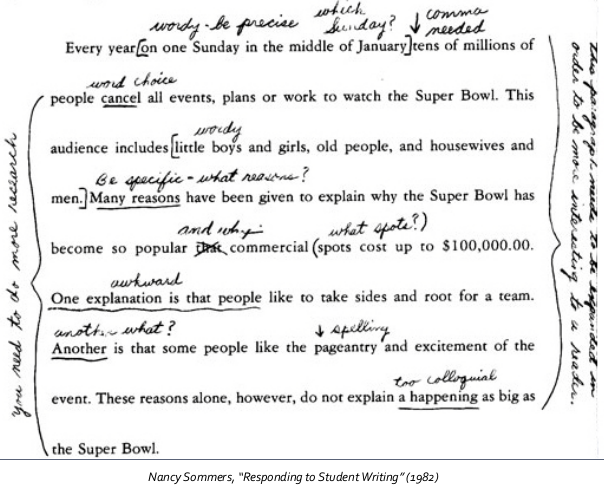
\includegraphics[scale=0.45]{feedback.png}
  \end{center}
}

\frame
{
  \ft{Type of Feedback}
  \bi
  \item End comments, as opposed to margin comments or in-text corrections.
  \item Minimal feedback that guides self discovery.
  \item Feedback sets priorities for students.
  \item Letters (about one page) are written to each group.
    \bi
    \item Thank students for the effort on this significant project.
    \item Commends students for aspects of the paper done well.
    \item Makes suggestions for revision priorities.
    \ei
  \ei
}

\frame
{
  \ft{Efficient Feedback}
  \bi
  \item We prepared a database of comments 
    \bi
    \item Comments are 1-3 sentences.
    \item Created over 50 to choose from.
    \ei
  \item Entered them all into text-expanding software
    \bi
    \item Software: Breevy for Windows, TextExpander for Mac.
    \item Each comment is mapped to a quick keystroke.
    \item Even the body of the letter is assigned a keystroke.
    \item Keystroke the body of the letter + Keystroke 3-5 comments.
    \item An entire letter can be written in a couple seconds with 4-6 keystrokes.
    \ei
  \ei
}

\frame[shrink]
{
  \ft{Example Letter}
\begin{scriptsize}
\begin{block}{}
Dear Members of Group 1,\\\vspace*{0.5pc}
I have reviewed the first draft of your introduction.  I think the following aspects represent the strongest qualities in your writing, and I encourage you keep these qualities in mind so that you retain them as you re-write for your final draft:\\\vspace*{0.5pc}

CITING LITERATURE:  You do a good job citing literature in your paper.  Your citations helped the reader understand the background and the importance of the issues your paper addresses.  Your use of citations support your narrative, as it should.\\\vspace*{0.5pc}

I think the following aspects of your paper could be improved.  Please consider these carefully and try to identify what in your paper you should rewrite to improve these aspects:\\\vspace*{0.5pc}

PURPOSE: More clearly state in the introduction exactly what the purpose of your paper is. In one or two sentences, describe compactly, yet precisely what your paper will accomplish – what question will you answer.\\\vspace*{0.5pc}

ORGANIZATION:  What is the argument or story you are trying to tell?  Outline or list the major points in order and make sure all your paragraphs are organized this way.\\\vspace*{0.5pc}

Thank you for the effort you put forth on this significant project.  Please let me what questions I can answer or what I can do further to help you improve your paper.   I look forward to reading your final draft.\\\vspace*{0.5pc}

Sincerely,\\
James Murray
\end{block}
\end{scriptsize}
}

\frame[label=body]
{
  \ft{Feedback Design}
  \bi
  \item Comments align to the learning goals for the assignment.
  \item Learning goals for the assignment align to CBA Writing Rubric
  \ei
}

\frame
{
  \ft{CBA Writing Traits and Assignment Learning Goals}
  \begin{block}{CBA Trait: Purpose and audience is addressed}
      \bi
      \item Clearly state the purpose of the research
      \item Ask all the relevant questions
      \ei
  \end{block}
  \begin{block}{CBA Trait: Organization of ideas and content is logical}
      \bi
      \item Communicate your message in a clear and meaningful way
      \ei
  \end{block}
  \begin{block}{CBA Trait: Content and ideas are developed}
      \bi
      \item Provide relevant background information
      \item Introduce your reader to how you answer your research question
      \ei
  \end{block}
}

\frame
{
  \ft{CBA Writing Traits and Assignment Learning Goals}

  \begin{block}{CBA Trait: Sources or evidence support ideas}
      \bi
      \item Use existing evidence to motivate your research
      \ei
  \end{block}
  \begin{block}{CBA Trait: Genre or disciplinary rules are followed}
      \bi
      \item Writing is professional and follows common rules for reporting research.
      \ei
  \end{block}
  \begin{block}{CBA Trait: Grammar, spelling and syntax is correct}
      \bi
      \item Communicate effectively by not distracting the reader with grammar and spelling errors.
      \ei
  \end{block}
}

\frame
{
  \ft{Comments for Feedback}
  \begin{block}{\footnotesize{1. Clearly state the purpose of the research}}
  \begin{tiny}
  \begin{columns}
    \column{2in}
    \textbf{Positive reinforcement:}\\
    DECISIONS:  Good work describing the types of decisions that could be better informed using the knowledge gained from your research project.  This helps your audience understand the purpose of your paper and helps motivate it.\\
PURPOSE: Good work clearly stating the purpose of your paper early in your introduction.  It is important to communicate this early so that the reader is drawn in and understands the context for the  discussion of the literature and the background information in your paper.\\\vspace*{0.5pc}
    \textbf{Suggestions for improvement:}\\
AUDIENCE / DECISIONS:  As you think about who your audience is (who would be interested in your paper), imagine that they are reading this paper voluntarily.  In the introduction, make it clear what kind of person / decision maker / researcher would be most interested in your work.  What could they do with the knowledge they gain from answering your research question?\\
CONTRIBUTION:  Are you trying to confirm or refute other contributions in the literature?  Are you trying to determine whether other findings in the literature hold for your population of interest?\\    
CONTRIBUTION:  Are you trying to confirm or refute other contributions in the literature?  Are you trying \\ \column{2in} to determine whether other findings in the literature hold for your population of interest?\\ 
DECISION PROCESS:  What kind of decisions would benefit from your research findings?  Think about adding this kind of discussion in your introduction.\\
PURPOSE:  Make sure the purpose of your paper comes out early in the introduction.  It need not be in the first paragraph, but soon after that may be appropriate.\\
PURPOSE: More clearly state in the introduction exactly what the purpose of your paper is.  In one or two sentences, describe compactly, yet precisely what your paper will accomplish – what question will you answer.\\
PURPOSE:  Your readers may not fully understand your purpose for doing this research project.  I suggest you write something early in the introduction to help your reader understand specifically what you will accomplish with this project.\\
PURPOSE:  Think about if what you describe as your purpose is really what you want to do.  Reflect on the issues that you discussed in your introduction.  The purpose of your paper should be to address the significance of those issues.\\
PURPOSE:  Be sure that the purpose of your paper is focused and communicated effectively early in the paper.  Are you making statements that are too broad or suggesting multiple purposes?
  \end{columns}

  \end{tiny}
  \end{block}
}

\frame
{
  \ft{Comments for Feedback}
  \begin{block}{\footnotesize{2. Ask all the relevant questions}}
  \begin{tiny}
  \begin{columns}
    \column{2in}
    \textbf{Positive reinforcement:}\\
   QUESTIONS / ISSUES:  Good job describing all the relevant questions or issues that you will investigate which are related to the overall purpose of your paper.\\\vspace*{0.5pc}
    \textbf{Suggestions for improvement:}\\
ASK THE RIGHT QUESTIONS:  Have all the right questions been asked in your introduction?  Think about the potential problems at the root of your \column{2in} issues, possible symptoms, and possible solutions to investigate.  Focus on the issues that the subsequent sections of your paper are likely to address.\\
QUESTIONS / ISSUES ESSENTIAL?  Are all the issues and questions you pose in the introduction essential?  Are there issues that the subsequent sections of your paper will not address?  If so, consider a more narrow focus for your introduction.  
  \end{columns}
  \end{tiny}
  \end{block}


  \begin{block}{\footnotesize{3. Provide relevant background information}}
  \begin{tiny}
  \begin{columns}
    \column{2in}
    \textbf{Positive reinforcement:}\\
BACKGROUND INFORMATION:  Good work laying down the right amount of background information to allow your reader to understand and appreciate the issues your paper will address.
\column{2in}
\textbf{Suggestions for improvement:}\\
BACKGROUND:  What other kind of background information would help your reader understand the context for and motivation of your research?

  \end{columns}
  \end{tiny}
  \end{block}
}

\frame{
  \ft{Comments for Feedback}
  \begin{block}{\footnotesize{4. Use evidence to motivate your research}}
  \begin{tiny}
  \begin{columns}
    \column{2in}
    \textbf{Positive reinforcement:}\\
CITING LITERATURE:  You do a good job citing literature in your paper.  Your citations helped the reader understand the background and the importance of the issues your paper addresses.  Your use of citations support your narrative, as it should.\\
CITING LITERATURE:  You have clearly used your literature review to provide background information and motivation for your research.\\
CITING LITERATURE:  You have clearly used your literature review to justify your hypotheses.\\\vspace*{0.5pc}

\textbf{Suggestions for improvement:}\\
LITERATURE:  Enhance the number and quality of citations to support the background information you do give, to provide more background information related to your research question and your methodology, and to help motivate the importance \column{2in} of your research project.\\
LITERATURE:  How do your references and background information work together to make a particular point?  Organize your literature review around the points that you are trying to make.\\
LITERATURE:  Does your literature review provide relevant background, or motivate your research or justify particular hypotheses?\\
LITERATURE:  Don’t just summarize the results of previous studies.  Use your literature review to illustrate the gaps in our knowledge and how your study will attempt to fill those gaps.\\
SUPPORTING EVIDENCE:  Make sure that you support your claims and/or background information by finding and citing appropriate evidence or literature.  Do not make the reader have to trust you at your word for background information you use which is not common knowledge.

  \end{columns}
  \end{tiny}
  \end{block}
}

\frame
{
  \ft{Comments for Feedback}

  \begin{block}{\footnotesize{5. Introduce your reader to how you will answer your research question}}
  \begin{tiny}
  \begin{columns}
    \column{2in}
\textbf{Positive reinforcement:}\\
METHODOLOGY: You do a good job briefly introducing your readers to how you will be answering your research question.  Your description has the right amount of detail, not so much as to repeat your methodology section.\\\vspace*{0.5pc}

\textbf{Suggestions for improvement:}\\
METHODOLOGY:  Do more to describe your methodology, but only briefly (a couple sentences to a paragraph, perhaps).  What will you do in this paper to answer your research question?  Most of these details should be put in your methodology section, but still, by the end of the introduction your reader should have a basic idea for how you plan to answer your research question.   Consider including the population, the use of a survey, and a general description of the types of questions in the survey.\\
METHODOLOGY:  Do more to describe your methodology, but only briefly (a couple sentences to a paragraph, perhaps).  What will you do in this paper to answer your research question?  \\\column{2in}
METHODOLOGY: Summarize for your reader the essential parts of the methodology you will use to answer your research question (for example, who will you study and how).\\
METHODOLOGY:  It is a good practice to introduce your readers to your methodology, but try to be more brief.  Briefly state who you will study and how.\\
METHODOLOGY:  It is a good practice to briefly introduce your readers to how you will be answering your research question.  This could be done with only two or three sentences, and not include much detail.  Your sentences could speak generally about the categories of variables you will collect and how it relates to your broader research question.  In your current draft, though, you include too much detail for an introduction.  Keep most of this discussion in the methodology section of your paper.\\
METHODOLOGY:  Think about if what you describe in your methodology is really what you want to do.  Reflect on the issues that you discussed in your introduction.  Your paper should address attempt to measure the significance of those issues.
  \end{columns}
  \end{tiny}
  \end{block}
}

\frame
{
  \ft{Comments for Feedback}

  \begin{block}{\footnotesize{6. Communicate your message in a clear and meaningful way}}
  \begin{tiny}
  \begin{columns}
    \column{2in}
\textbf{Positive reinforcement:}\\
CONCISENESS: Good work writing your paper in a concise way.  You do a good job of quickly getting to the point without failing to discuss essential issues or details.
OPENING:  You have a good opening.  It draws the reader in and it is relevant to the rest of your paper.  A good opening not only draws the reader in, but what is covered in the opening should be addressed satisfactorily by the end of the paper.\\
ORGANIZATION:  You do a good job meaningfully organizing your writing along important themes.  For the most part, each subsequent paragraph speaks to a specific purpose that clearly contributes to an overall purpose of the paper, and the movement from one purpose to another is logical and meaningful.\\
TRANSITIONS:  Good work on your transitions from one paragraph to the next and from one idea/topic to the next.  Good transitions connect paragraphs to each other, allows the reader to understand how the paragraphs are related to one another and how they jointly build to a larger point. \\\vspace*{0.5pc}

\textbf{Suggestions for improvement:}\\
CONCISENESS: Are there one or two places where your writing can be made more concise?  Carefully read over your work and consider one or two ways to make it more concise.\\ \column{2in}
CONCISENESS:  Think about how you can make this writing more concise.  Think about if there any sentences or paragraphs that can be removed without losing quality or important evidence or details and still keep to the purpose of your paper.  Think about whether there are sentences that can be combined more concisely, or if individual sentences can be rewritten more concisely without removing their meaning.\\
OPENING:  The opening of your paper is too general, or it is not immediately applicable to your particular paper.  Consider writing an opening more closely related to the purpose of your paper.  Use an opening that draws the reader in and that raises an issue that you know your paper will satisfactorily address.\\
ORGANIZATION:  Think about how you want to organize your introduction.  I suggest writing an outline for the main points of your story, and be sure that each paragraph stays focused on a particular point.  While there may be some overlap, your introduction could be well organized by focusing first on your research question, then provide background and motivation, and then briefly describe your methodology.\\
ORGANIZATION:  What is the argument or story you are trying to tell?  Outline or list the major points in order and make sure all your paragraphs are organized this way.\\
  \end{columns}
  \end{tiny}
  \end{block}
}

\frame
{
  \ft{Comments for Feedback}
  \begin{block}{\footnotesize{6. Communicate your message in a clear and meaningful way (continued)}}
\begin{tiny}
\begin{columns}
\column{2in}
\textbf{Suggestions for improvement (continued):}\\
ORGANIZATION:  Work to improve how this writing is organized.  Each paragraph should speak to only one point, and the purpose of each paragraph should build on the previous one and all should contribute to the overall purpose of the writing.  Make sure the movement from one purpose is logical and meaningful.  Also, think about whether you have two or three larger purposes in this piece, and organize your writing around these. \\ 
ORGANIZATION / OUTLINE: If you have not already done so, consider making an outline of your paper, with each paragraph an element in your outline.   Can \column{2in} you see ways to improve the organization?\\
TRANSITIONS:  Reread your work and think about if there are any paragraphs that have weak or choppy transitions from the previous paragraph.  Consider ways to improve these transitions.\\
TRANSITIONS:  Work on your transitions from one paragraph to the next or one idea/topic to the next.  Good transitions connect paragraphs to each other, allow the reader to understand how the paragraphs are related to one another and how they jointly build to a larger point.  Good transitions also  allow the narration to flow more smoothly, and sound less like a list of related ideas.\\
\end{columns}
\end{tiny}
\end{block}
}

\frame
{
  \ft{Comments for Feedback}
  \begin{block}{\footnotesize{7. Communicate effectively}}
\begin{tiny}
\begin{columns}
\column{2in}
\textbf{Positive reinforcement:}\\
CITATION STYLE: You have been consistent in the citation style you have used.  If additional questions come up, the following website has an APA and MLA formatting and style guide which is easy to use  http://owl.english.purdue.edu/  Use this resource to ensure consistency.\\\vspace*{0.5pc}
\textbf{Suggestions for improvement:}\\
CITATION STYLE:  It is important to be consistent in the citation style.   Refer to http://owl.english.purdue.edu/owl/resource/560/02/ for APA citation style.\\
CITATION STYLE:  Make sure you cite papers correctly using only the author(s) last name(s) and year (eg: Smith (1990) finds that…).  You likely should not include author’s first names, the journal title, the paper title, etc.  All this information will be in the bibliography of the paper.  The following website describes APA format for citing in the text of your paper: http://owl.english.purdue.edu/owl/resource/560/02/.  Use this resource to ensure consistency.\\
CITATION:  In addition to providing an in-text citation when you quote an author, it is also necessary to paraphrase the persons’ idea.  Refer to \column{2in} http://owl.english.purdue.edu/ and consult the APA or MLA formatting and style guide.\\ 
DIFFICULT TO FOLLOW:  In some instances your writing is difficult to follow.  Re-read your own work and make sure you can follow through the sentences and your train of thought.  It would be a good idea to also have another member of your group who did not write the piece read over your work.  Ask them to point out sentences or sections of the paper where it is difficult to follow.\\
GRAMMAR / SPELLING / PUNCTUATION:  I found some errors in grammar, spelling, or punctuation.  Reread your work and see if you can find and fix these (or even better, ask a friend to do it!).\\ 
GRAMMAR / SPELLING / PUNCTUATION:  I found several errors in grammar, spelling, or punctuation (note, spell checkers do not always pick up incorrect uses of a word (for  example ``their,'' ``there,'' and ``they’re'' or ``affect'' versus ``effect'').  After rewriting your introduction, please look out more carefully for these.  I strongly suggest asking a classmate to double check your work (and perhaps you could return the favor).  It is common to read in your mind what you intended to write, making it difficult to catch your own grammar mistakes, but easier for others to catch them.  \\
\end{columns}
\end{tiny}
\end{block}
}

\frame
{
  \ft{Comments for Feedback}
  \begin{block}{\footnotesize{7. Communicate effectively (continued)}}
\begin{tiny}
\begin{columns}
\column{2in}
\textbf{Suggestions for improvement (continued):}\\
HYPERBOLE:  Be careful with your use of hyperbole.  It can be acceptable to use language that argues a particular viewpoint or side, but using it is much harder to provide evidence, much less proof, for statements that include hyperbole.  Using this language can also turn off readers who may not agree with the extremity of your statements.  \\
QUOTES:  When you directly quote someone, it is necessary to provide an in-text citation to identify the source. Refer to http://owl.english.purdue.edu/ and consult the APA or MLA formatting and style guide.\\
QUOTES:  Only directly quote another author if you find paraphrasing it yourself is not adequate.  This should only happen when the original author used words that were particularly clever or eloquent.  Another reason a quote may be if it is important to point out that the particular phrase you quote was actually stated by the particular person, for example if the person is an important public figure, and the \column{2in} phrase is evidence for some point of view.  Finally, if you do use direct quotations, you still have to paraphrase anyway.  Your writing should still sound complete and coherent even if the reader glances over the precise quotation.\\
VERB TENSE:  Make sure verb tense agrees throughout the paper, and stick with present tense when possible.  Do not switch from one tense to another in a sentence, in a paragraph, or even in the whole document, unless the timing of an action you are describing demands you do.  Be sure to also cite literature in present tense, as in ``Smith (1990) finds that…''  instead of ``Smith (1990) found that…''\\
ACTIVE / PASSIVE VOICE:  Try to always write in active voice.  Active voice means writing sentences as ``subject does verb to object,'' as in, ``Jenny throws the ball.''  Passive voice sounds like ``object has verb acted upon by subject,'' as in, ``The ball is thrown by Jenny.''  Look through your writing and rewrite passive voice sentences to active voice.
\end{columns}
\end{tiny}
\end{block}
}

\frame
{
  \ft{Classroom Observation Day}
  \bi
  \item Week following their initial submission of the introduction section of their final paper.
  \item Self-evaluation:
    \bi
    \item Students reflect on 7 learning goals, give themselves scores for each.
    \item Suggest revision priorities
    \ei
  \item Feedback letters are handed out
  \item Students respond with revisions or plans - team of instructors observed students conversations.
    \bi
    \item Fall 2012: Students filled out a revision plan worksheet = disaster
    \item Spring 2013: Students were in a computer lab, asked them to use the time to start working on their revisions.
    \ei
  \ei
}

\frame
{
  \ft{Fall 2012 Activity}
\begin{footnotesize}
Read over the feedback you received on your writing and think about specific revisions you
would like to make. In the first column describe some details about what you will write or what
you will change that will give you a road map to follow as you start writing again. In the second
column describe specifically 1) what you will do and 2) who will complete these tasks.\\

\begin{center}
\begin{tabular}{|c|c|} \hline
\textbf{~~~~~Needs Revision~~~~~} & \textbf{~~~~~~~Action Steps~~~~~~~} \\ \hline
& \\ & \\ & \\
 & \\ \hline
& \\ & \\ & \\
 & \\ \hline
& \\ & \\ & \\
 & \\ \hline
\end{tabular}
\end{center}
\end{footnotesize}
}

\frame[shrink]
{
  \ft{Spring 2013 Activity}
  \begin{block}{Focus on Purpose}
    Evaluate if the introduction speaks a focused, unified, coherent, message.
  \end{block}

  \begin{block}{Discussion Prompts}
    \bi
    \item Is there a clear communication of the purpose of your research project early in the introduction? (LO 1)
    \item Does your background information contribute directly to your purpose?  Do marginally related topics detract from your purpose? (LO 3)
    \item Do your citations contribute directly to your purpose?  Do marginally related topics detract from your purpose? (LO 4)
    \item Do you have a brief description of your methodology that convinces your audience you are going to take steps to accomplish precisely what you communicated as your purpose for the research? (LO 5)
    \ei
  \end{block}
}

\frame
{
  \ft{Observations}
  \begin{block}{Many students resisted feedback}
    \bi
    \item Some students postponed doing meaningful work.
    \item Some students ignored feedback and discussion prompts.
    \item Some students regarded the paper as complete.
    \item Even students that identified significant revisions concentrated on local corrections.
    \ei
  \end{block}

  \begin{block}{Many students already identified shortcomings}
    \bi
    \item They knew the problem, but not how to address it.
    \item Could more useful comments be constructed that:
      \bi
      \item Suggest a short brainstorming exercise?
      \item Pose a question to the students, such that the students' answers suggest how the paper be rewritten?
      \ei
    \item Most likely need to complement letters with face-to-face consultations.
    \ei
  \end{block}
}

\frame
{
  \ft{Comment-Specific Observations}
  \bi
  \item Many students did not understand comments on purpose.
    \bi
    \item Students reported a specific purpose early in intro, nonetheless spoke to multiple purposes.
    \item Students brought up background information that addresses issues only related to purpose.
    \item Students stated a purpose that was not appropriate.
    \ei
  \item Student perceived some comments as contradictory.
    \bi
    \item Example: Good organization, difficult to follow.
    \ei
  \item Discussion prompts in Spring 2013 may make valuable feedback.
  \ei
}

\frame
{
  \ft{Some Successes!}
  \begin{block}{One good discussion in Spring 2013}
    Discussed the paper as one connected product, individual components speaking to one purpose.  They connected individual comments to the one purpose.
  \end{block}

  \begin{block}{Several comments were well understood}
    \bi
    \item Improve organization, consider making an outline.
    \item Improve quantity of citations and background evidence.
    \item Improve transitions.
    \item Introduce your methodology.
    \item Grammar / spelling issues.
    \ei
  \end{block}
}

\frame
{
  \ft{Conclusions}
  \begin{block}{Three out of four isn't bad!}
    \be
    \item Efficient feedback mechanism. 
\includegraphics[scale=0.04]{check.jpg} 
    \item Effective feedback - No direct evidence.  Working on it! 
\includegraphics[scale=0.04]{xmark.jpg} 
    \item Feedback consistent with expectations. 
\includegraphics[scale=0.04]{check.jpg} 
    \item Process conducive to pedagogical growth. 
\includegraphics[scale=0.04]{check.jpg} 
    \ee
  \end{block}

  \begin{block}{Potential Plan Moving Forward}
    \be
    \item Prepare students for \textit{rewriting}.
    \item Students evaluate their work using the learning goals.
    \item Hand out feedback letters.
    \item Have students consider prompts regarding purpose.
    \item Face-to-face consultations.
    \ee
  \end{block}
}

\frame
{
  \frametitle{~}
  \begin{center}\LARGE{\textbf{Thank You}}\end{center}
}



\end{document}

